% EN3160 Assignment 2 - compact report styled after the supplied reference .tex
\documentclass[9pt,a4paper]{article}

\usepackage[a4paper,left=0.72in,right=0.72in,top=0.68in,bottom=0.72in]{geometry}
\usepackage[T1]{fontenc}
\usepackage{lmodern}
\usepackage{graphicx}
\usepackage{float}
\usepackage{booktabs}
\usepackage{tabularx}
\usepackage{array}
\usepackage{amsmath,amssymb}
\usepackage{enumitem}
\usepackage{caption}
\usepackage{subcaption}
\usepackage{setspace}
\usepackage{titlesec}
\usepackage{fancyhdr}
\usepackage{url}
\usepackage{xcolor}
\usepackage{hyperref}
\usepackage{tikz}
\usepackage{listings}

\definecolor{navy}{HTML}{17324D}
\definecolor{blue}{HTML}{2F6B97}
\definecolor{pale}{HTML}{F1F5F8}
\definecolor{muted}{HTML}{5D6B76}
\definecolor{grid}{HTML}{D3DEE7}

% Edit these three fields if your submission details differ.
\newcommand{\StudentName}{Dilhara D.S.}
\newcommand{\IndexNumber}{230147L}
\newcommand{\GitHubProfile}{https://github.com/sachi1645/Fitting-and-Alignment}
% Generated from results/ by src/make_report.py. Do not edit by hand.
\newcommand{\QOneDetectionCount}{271}
\newcommand{\QOneScaleCount}{32}
\newcommand{\QOneSigmaRange}{0.5--8.0}
\newcommand{\QOneThreshold}{0.06}
\newcommand{\QOneWindow}{7\times7}
\newcommand{\QOneRoi}{180}
\newcommand{\QOneYellowFraction}{0.28}
\newcommand{\QOneContrast}{8.0}
\newcommand{\QOneLargestRows}{%
1 & 282 & 338 & 7.32 & 10.35 & 0.349\\
2 & 79 & 258 & 6.69 & 9.46 & 0.178\\
3 & 106 & 255 & 6.12 & 8.65 & 0.362\\
4 & 179 & 327 & 6.12 & 8.65 & 0.345\\
5 & 178 & 261 & 5.59 & 7.91 & 0.353\\
6 & 339 & 206 & 5.59 & 7.91 & 0.098\\
7 & 29 & 272 & 5.12 & 7.23 & 0.151\\
8 & 189 & 240 & 4.68 & 6.62 & 0.362\\
}
\newcommand{\QTwoLineInliers}{56/100}
\newcommand{\QTwoLineNormal}{0.715649, 0.698460}
\newcommand{\QTwoLineNorm}{1.000000}
\newcommand{\QTwoLineD}{1.561775}
\newcommand{\QTwoLineSlope}{-1.024609}
\newcommand{\QTwoLineIntercept}{2.236025}
\newcommand{\QTwoCircleInliers}{42}
\newcommand{\QTwoCircleCenter}{1.817367, 3.089484}
\newcommand{\QTwoCircleRadius}{9.888575}
\newcommand{\QTwoLineComposition}{50 true-line + 6 true-circle points}
\newcommand{\QTwoCircleComposition}{42 true-circle + 0 true-line points}
\newcommand{\QTwoCircleFirst}{57 points (48 true-circle and 9 line points)}
\newcommand{\QTwoCircleFirstLineInliers}{41}
\newcommand{\QFourMetricRows}{%
AAAA1 & 51 & 18 & 28.8 & 107\\
ADAD1 & 369 & 194 & 31.2 & 92\\
AECC2 & 4322 & 3847 & 3.5 & 9\\
AECC3 & 5629 & 5006 & 3.2 & 8\\
AECC4 & 3830 & 3402 & 4.0 & 10\\
}
\newcommand{\QFourHighDiffImages}{AAAA1 and ADAD1}


\hypersetup{colorlinks=true,linkcolor=navy,urlcolor=blue,pdftitle={EN3160 Assignment 2 - Fitting and Alignment},pdfauthor={\StudentName}}
\setlength{\parindent}{0pt}
\setlength{\parskip}{0.25em}
\setstretch{1.02}
\setlength{\tabcolsep}{3.4pt}
\renewcommand{\arraystretch}{1.14}
\captionsetup{font=footnotesize,labelfont=bf,justification=centering,skip=3pt}
\titleformat{\section}{\normalfont\bfseries\large\color{navy}}{\thesection}{0.6em}{}
\titlespacing*{\section}{0pt}{5pt}{2pt}
\titleformat{\subsection}{\normalfont\bfseries\normalsize\color{blue}}{\thesubsection}{0.6em}{}
\titlespacing*{\subsection}{0pt}{4pt}{1pt}
\lstset{basicstyle=\ttfamily\scriptsize,backgroundcolor=\color{pale},frame=single,rulecolor=\color{grid},breaklines=true,columns=fullflexible,xleftmargin=4pt,xrightmargin=4pt,aboveskip=3pt,belowskip=3pt}

% Draw the page frame at shipout so it stays outside the text/footer area.
\AddToHook{shipout/background}{%
  \begin{tikzpicture}[remember picture,overlay]
    \draw[line width=0.45pt,color=black!75]
      ([xshift=0.25cm,yshift=-0.25cm]current page.north west)
      rectangle
      ([xshift=-0.25cm,yshift=0.25cm]current page.south east);
  \end{tikzpicture}%
}

\pagestyle{fancy}
\fancyhf{}
\fancyhead[L]{\textcolor{navy}{\small\bfseries University of Moratuwa | EN3160}}
\fancyhead[R]{\textcolor{muted}{\small Assignment 2}}
\renewcommand{\headrulewidth}{0.35pt}
\renewcommand{\headrule}{\hbox to\headwidth{\color{grid}\leaders\hrule height \headrulewidth\hfill}}
\fancyfoot[L]{\textcolor{muted}{\scriptsize\StudentName\ | \IndexNumber}}
\fancyfoot[R]{\textcolor{muted}{\scriptsize Page \thepage\ of 4}}
\renewcommand{\footrulewidth}{0pt}
\setlength{\headheight}{13pt}

\begin{document}

% PAGE 1 -------------------------------------------------------------------
\begin{center}
{\Large\bfseries\color{navy} EN3160 -- Fitting and Alignment}\par
{\large\bfseries Assignment 2 Report}\par
{\small Student: \StudentName \quad | \quad Index: \IndexNumber \quad | \quad GitHub: \href{\GitHubProfile}{\texttt{github.com/sachi1645/Fitting-and-Alignment}}}
\end{center}
\vspace{-2pt}\hrule\vspace{4pt}

\section*{1. Laplacian-of-Gaussian blob detection}
The supplied sunflower photograph is loaded with \texttt{cv2.IMREAD\_REDUCED\_COLOR\_4}, giving a $360\times360$ image. For each Gaussian scale, the detector evaluates the absolute scale-normalised Laplacian,
\[
L(x,y,\sigma)=\left|\sigma^2\nabla^2(G_\sigma * I)(x,y)\right|,\qquad r\approx\sqrt{2}\,\sigma.
\]
Local maxima are extracted in the spatial-scale response stack and duplicate scale-space candidates are suppressed. To focus on sunflower heads rather than leaves and tree texture, candidates are restricted to $y\ge\QOneRoi$ and validated by the yellow-petal fraction and grayscale contrast of an annulus around a darker centre. No \texttt{cv2.HoughCircles} call is used.

\textbf{Selected parameters.} \QOneScaleCount\ logarithmically spaced scales, $\sigma=\QOneSigmaRange$ reduced-image pixels; response threshold $\QOneThreshold$; spatial neighbourhood $\QOneWindow$; yellow annulus fraction $\ge\QOneYellowFraction$; ring-minus-centre grayscale contrast $\ge\QOneContrast$. The output draws every validated detection, not just the largest few.

\vspace{1pt}
\begin{minipage}[t]{0.51\textwidth}
\vspace{0pt}
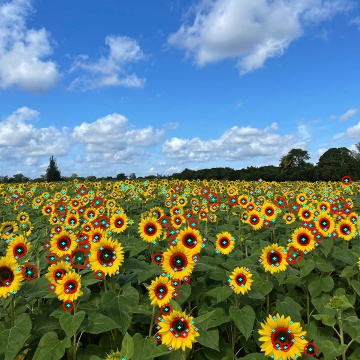
\includegraphics[width=\linewidth]{report_assets/q1_sunflower.jpg}
\captionof{figure}{LoG detections over the course sunflower image. All \QOneDetectionCount\ validated candidates are drawn.}
\end{minipage}\hfill
\begin{minipage}[t]{0.46\textwidth}
\vspace{0pt}
\textbf{Largest detected circles}\par
\small Centres and radii use reduced-image pixels; multiply by four to convert to original-image coordinates.
\vspace{2pt}
{\scriptsize
\begin{tabularx}{\linewidth}{@{}r r r r r >{\raggedleft\arraybackslash}X@{}}
\toprule
\# & $x$ & $y$ & $\sigma$ & radius & resp.\\
\midrule
\QOneLargestRows
\bottomrule
\end{tabularx}}
\vspace{3pt}
\textbf{Interpretation.} Extending the scale range down to $0.5$ px recovers smaller flower heads that were missed by the original $1.3$ px lower limit. Colour/contrast validation rejects many foliage responses. The detector still finds candidate blobs rather than semantically segmenting every flower: occlusion, overlapping heads, shadows and similar leaf texture can cause misses or false positives.
\end{minipage}

\vspace{2pt}
\begin{lstlisting}
response = abs(sigma**2 * gaussian_laplace(gray, sigma))
peaks = local maxima in the spatial-scale response stack
radius = sqrt(2) * sigma
\end{lstlisting}

% PAGE 2 -------------------------------------------------------------------
\newpage
\section*{2. RANSAC line and circle fitting}
Listing 1 is reproduced with a fixed random seed and 100 points: 50 noisy circle points with ground truth centre $(2,3)$ and radius $10$ (radial noise standard deviation $0.625$), and 50 noisy line points from $y=-x+2$ (vertical noise standard deviation $1$). The hand-coded RANSAC line model uses a unit normal $[a,b]^T$ and perpendicular distance residuals. Its consensus is refitted using total least squares; those inliers are removed before circle RANSAC uses three-point samples and minimises radial residuals on the consensus.

\begin{minipage}[t]{0.61\textwidth}
\vspace{0pt}
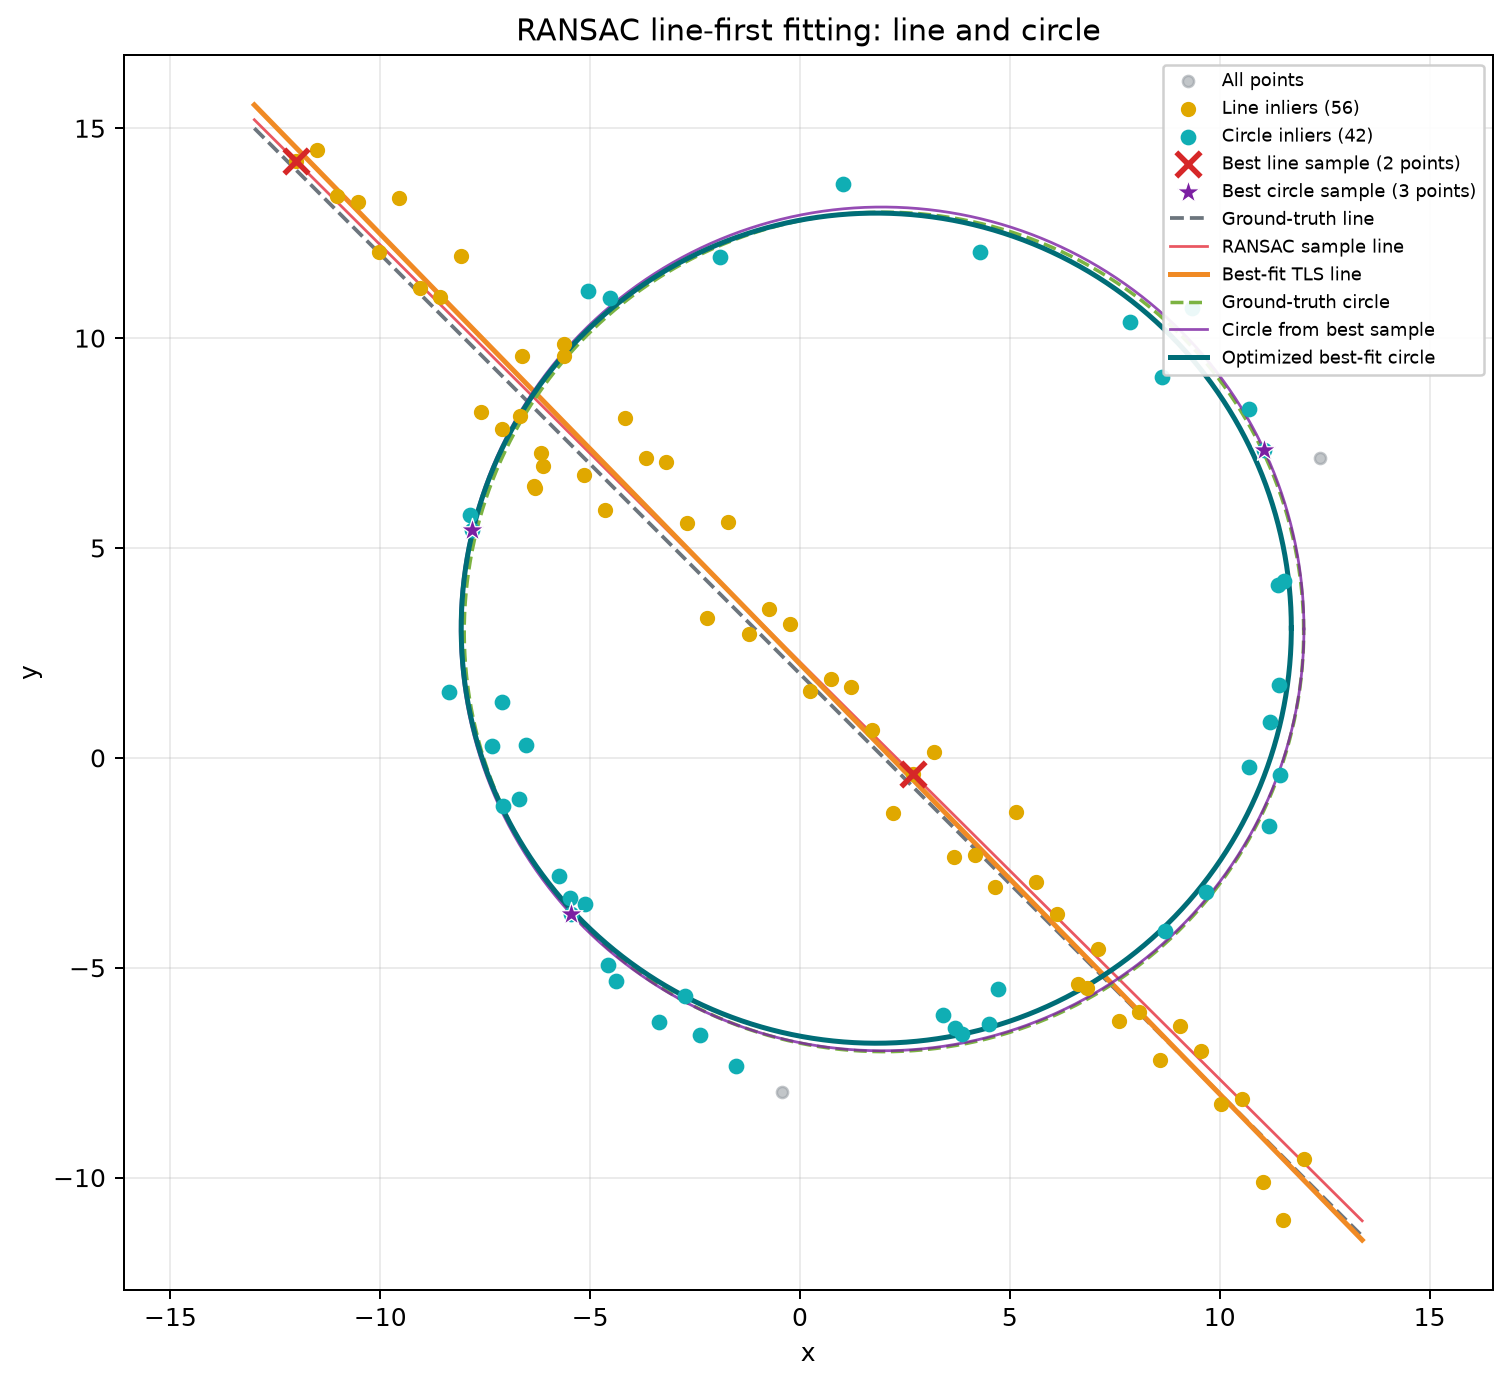
\includegraphics[width=\linewidth]{report_assets/q2_ransac.png}
\captionof{figure}{Point set, ground-truth and fitted models, selected minimal samples and consensus sets.}
\end{minipage}\hfill
\begin{minipage}[t]{0.36\textwidth}
\vspace{0pt}
\textbf{RANSAC settings}\par
\small
\begin{tabularx}{\linewidth}{@{}lX@{}}
\toprule
Line & 2,500 iterations; threshold $1.7$; minimum consensus $35$\\
Circle & 4,500 iterations; threshold $1.25$; minimum consensus $32$\\
\bottomrule
\end{tabularx}
\vspace{4pt}
\textbf{Estimated models}\par
\begin{tabularx}{\linewidth}{@{}lX@{}}
\toprule
Line normal & $(\QTwoLineNormal)$\\
Normal norm & $\QTwoLineNorm$\\
Line $d$ & $\QTwoLineD$\\
Line $y=mx+b$ & $m=\QTwoLineSlope$, $b=\QTwoLineIntercept$\\
Circle centre & $(\QTwoCircleCenter)$\\
Radius & $\QTwoCircleRadius$\\
\bottomrule
\end{tabularx}
\end{minipage}

\vspace{4pt}
\textbf{Ground truth versus estimate}
\begin{center}
\small
\begin{tabular}{@{}lll@{}}
\toprule
Parameter & Ground truth & Estimate\\
\midrule
Line slope & $-1.0000$ & $\QTwoLineSlope$\\
Line intercept & $2.0000$ & $\QTwoLineIntercept$\\
Circle centre & $(2,3)$ & $(\QTwoCircleCenter)$\\
Circle radius & $10.0000$ & $\QTwoCircleRadius$\\
\bottomrule
\end{tabular}
\end{center}

\textbf{Consensus and interpretation.} The line-first fit returns \QTwoLineInliers\ line inliers (\QTwoLineComposition). After removing them, the circle fit returns \QTwoCircleInliers\ circle inliers (\QTwoCircleComposition). The estimated circle centre is approximately $0.204$ units from the true centre and the radius error is approximately $0.111$. The fitted line is close to the ground truth; residual differences arise from noise and random sampling.

\textbf{(d) If the circle is fitted first.} Circle-first RANSAC returns \QTwoCircleFirst. The remaining 43 points then yield \QTwoCircleFirstLineInliers\ true-line inliers. Therefore, model order changes the assignment of ambiguous points: the circle can absorb points from the line before the line fit ever sees them. Sequential RANSAC is effective here because the selected line consensus is removed before estimating the circle.

% PAGE 3 -------------------------------------------------------------------
\newpage
\section*{3. Homography and perspective overlay}
A homography projects a planar overlay into a four-corner quadrilateral in the background. For each example, source corners are the overlay image corners; destination points are clicked or specified in the clockwise order top-left, top-right, bottom-right, bottom-left. The projective transform is computed with \texttt{cv2.getPerspectiveTransform} and applied with \texttt{cv2.warpPerspective}. A warped validity mask limits blending to the overlay area so unfilled pixels do not blacken the background.

\begin{figure}[H]
\centering
\begin{subfigure}[t]{0.485\textwidth}
\centering
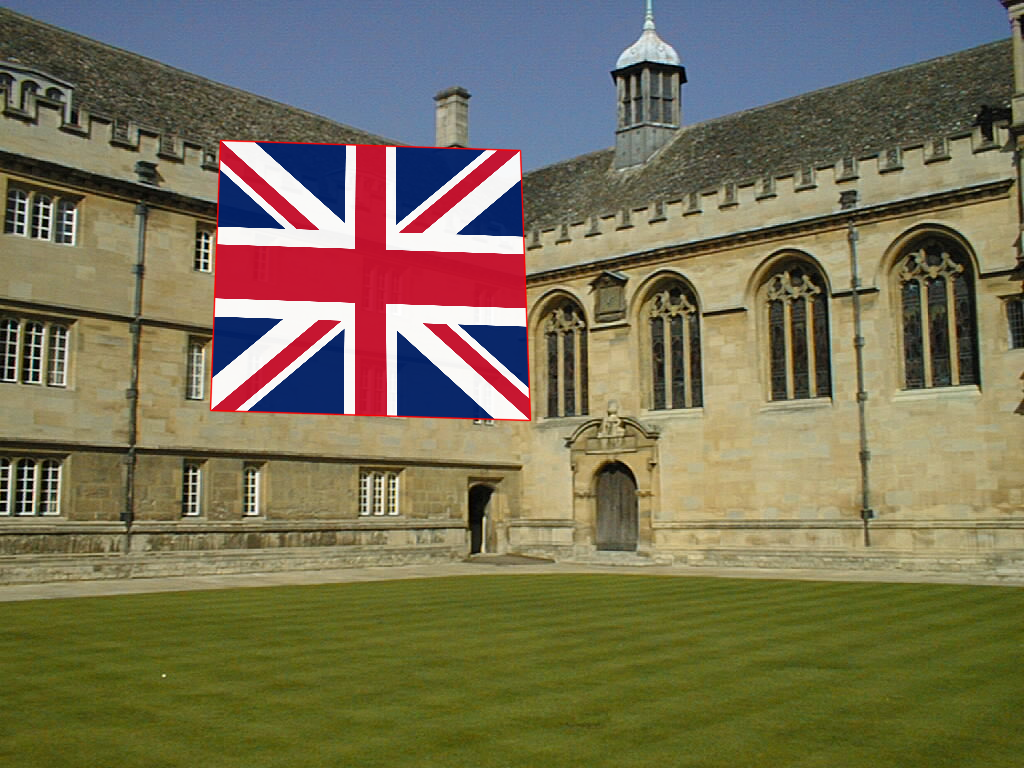
\includegraphics[width=\linewidth]{report_assets/q3_flag.png}
\caption{Union Jack on the Wadham College facade.}
\end{subfigure}\hfill
\begin{subfigure}[t]{0.485\textwidth}
\centering
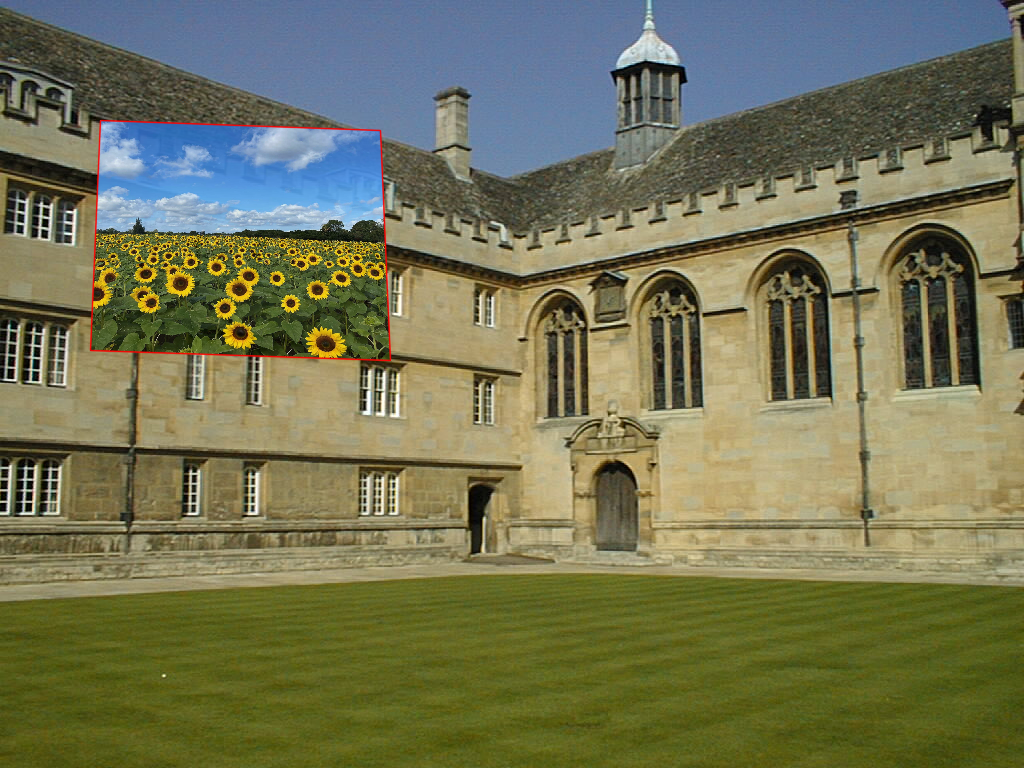
\includegraphics[width=\linewidth]{report_assets/q3_poster.png}
\caption{Sunflower image placed as a small poster.}
\end{subfigure}
\caption{Two overlays warped onto planar regions in the same supplied architecture image.}
\end{figure}

\textbf{Destination quadrilaterals (TL, TR, BR, BL)}
\begin{center}
\small
\begin{tabularx}{0.96\textwidth}{@{}l X X@{}}
\toprule
Setting & Example 1: flag & Example 2: poster\\
\midrule
Background & \texttt{wadham.jpg} & \texttt{wadham.jpg}\\
Overlay & \texttt{flag.png} & sunflower field photo\\
Coordinates & $(220,250),(480,277),(474,410),(215,394)$ & $(72,295),(185,303),(181,382),(69,374)$\\
Blend $\alpha$ & $0.97$ & $0.97$\\
\bottomrule
\end{tabularx}
\end{center}

\textbf{Rationale and discussion.} A flag is a recognisable graphic for a large facade area, whereas the sunflower photograph demonstrates a smaller poster. The projected corners follow each selected quadrilateral, and the validity mask preserves the rest of the architecture. Correct point order is crucial; misordered corners can rotate, flip or twist the overlay. A single homography models one plane, so it cannot accurately handle protruding objects or a target surface with substantial depth variation. The interactive script also permits selecting four new corners for other image pairs.

% PAGE 4 -------------------------------------------------------------------
\newpage
\section*{4. SIFT PCB alignment and difference images}
The reference is \texttt{AECC1.jpg}. SIFT keypoints/descriptors are matched by \texttt{cv2.BFMatcher} using the L2 metric. Lowe's ratio test ($0.75$) removes ambiguous pairs; RANSAC estimates a homography with a $5$ px reprojection threshold. Each test PCB is warped to the template dimensions. The absolute grayscale difference is computed only in the valid warped overlap, excluding uncovered black borders from its statistics.

\begin{minipage}[t]{0.43\textwidth}
\vspace{0pt}
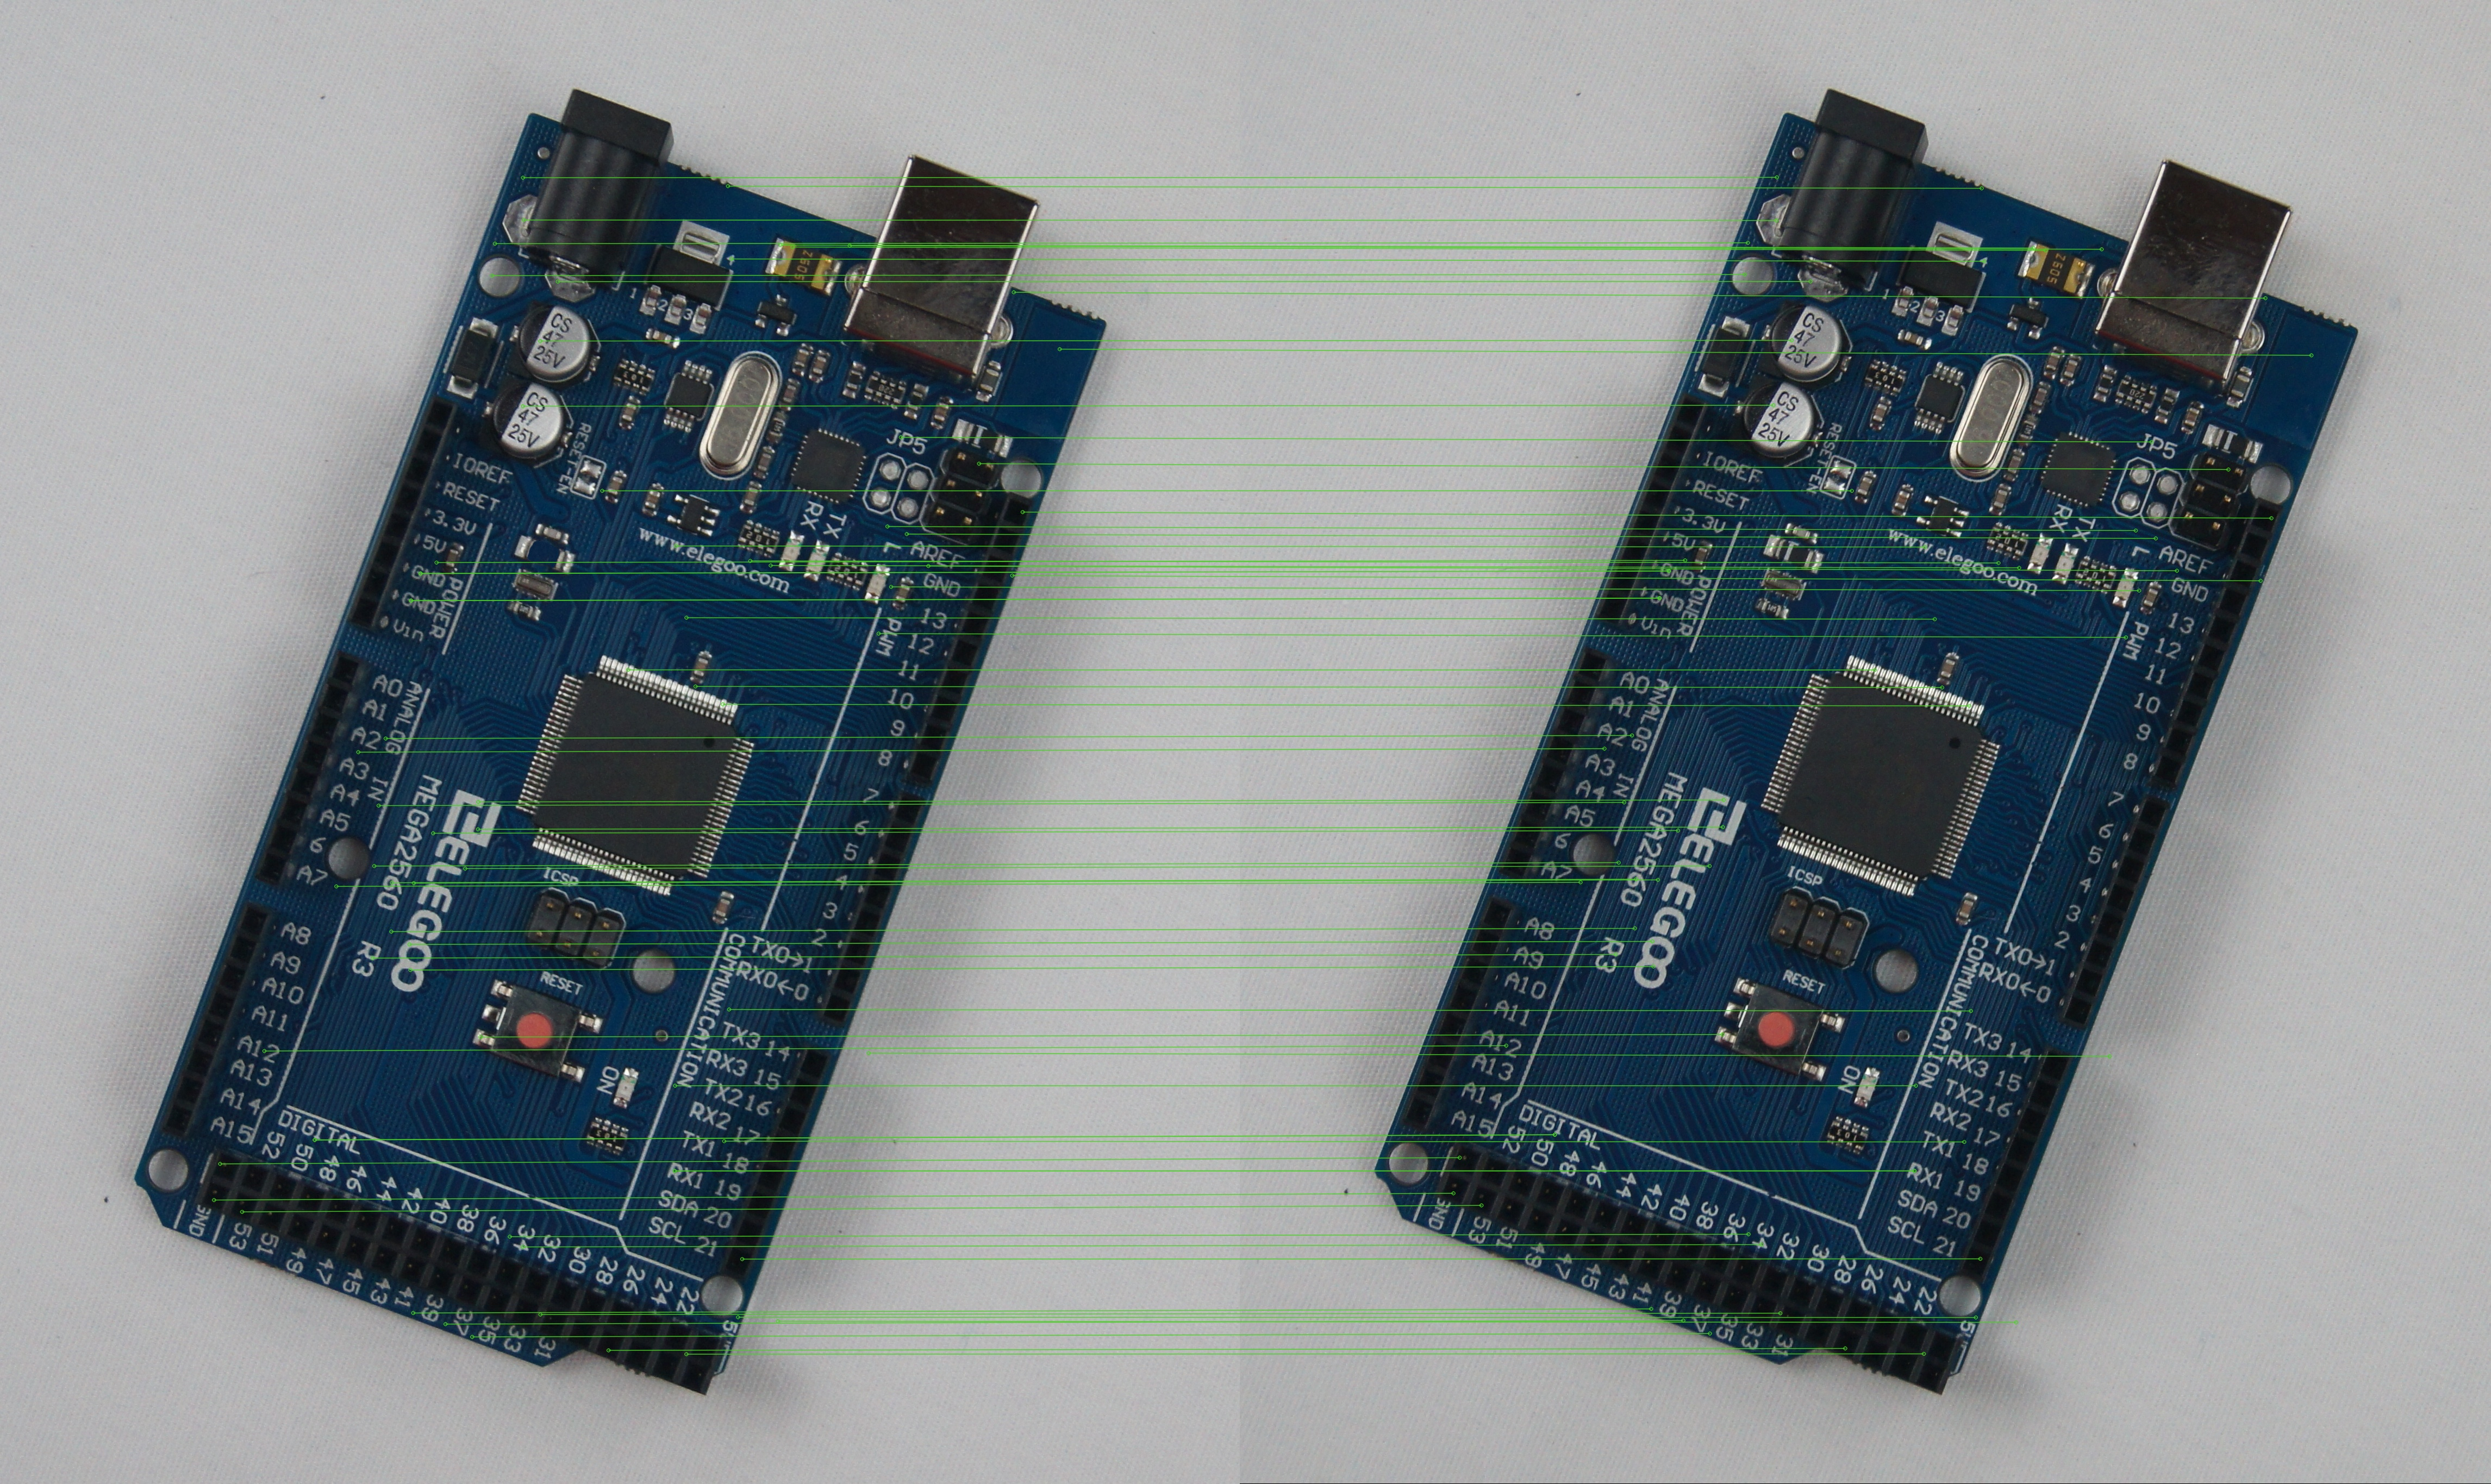
\includegraphics[width=\linewidth]{report_assets/q4_matches.jpg}
\captionof{figure}{Example SIFT inlier matches: AECC2 to AECC1.}
\end{minipage}\hfill
\begin{minipage}[t]{0.54\textwidth}
\vspace{0pt}
\textbf{Alignment and grayscale difference metrics}\par
\scriptsize
\begin{tabularx}{\linewidth}{@{}l r r r r@{}}
\toprule
Image & Matches & Inliers & Mean $|\Delta|$ & 95th pct.\\
\midrule
\QFourMetricRows
\bottomrule
\end{tabularx}
\end{minipage}

\vspace{1pt}
\textbf{Difference heatmaps} (all test images; brighter/hotter regions indicate larger local differences)

\begin{center}
\begin{minipage}[t]{0.32\textwidth}\centering
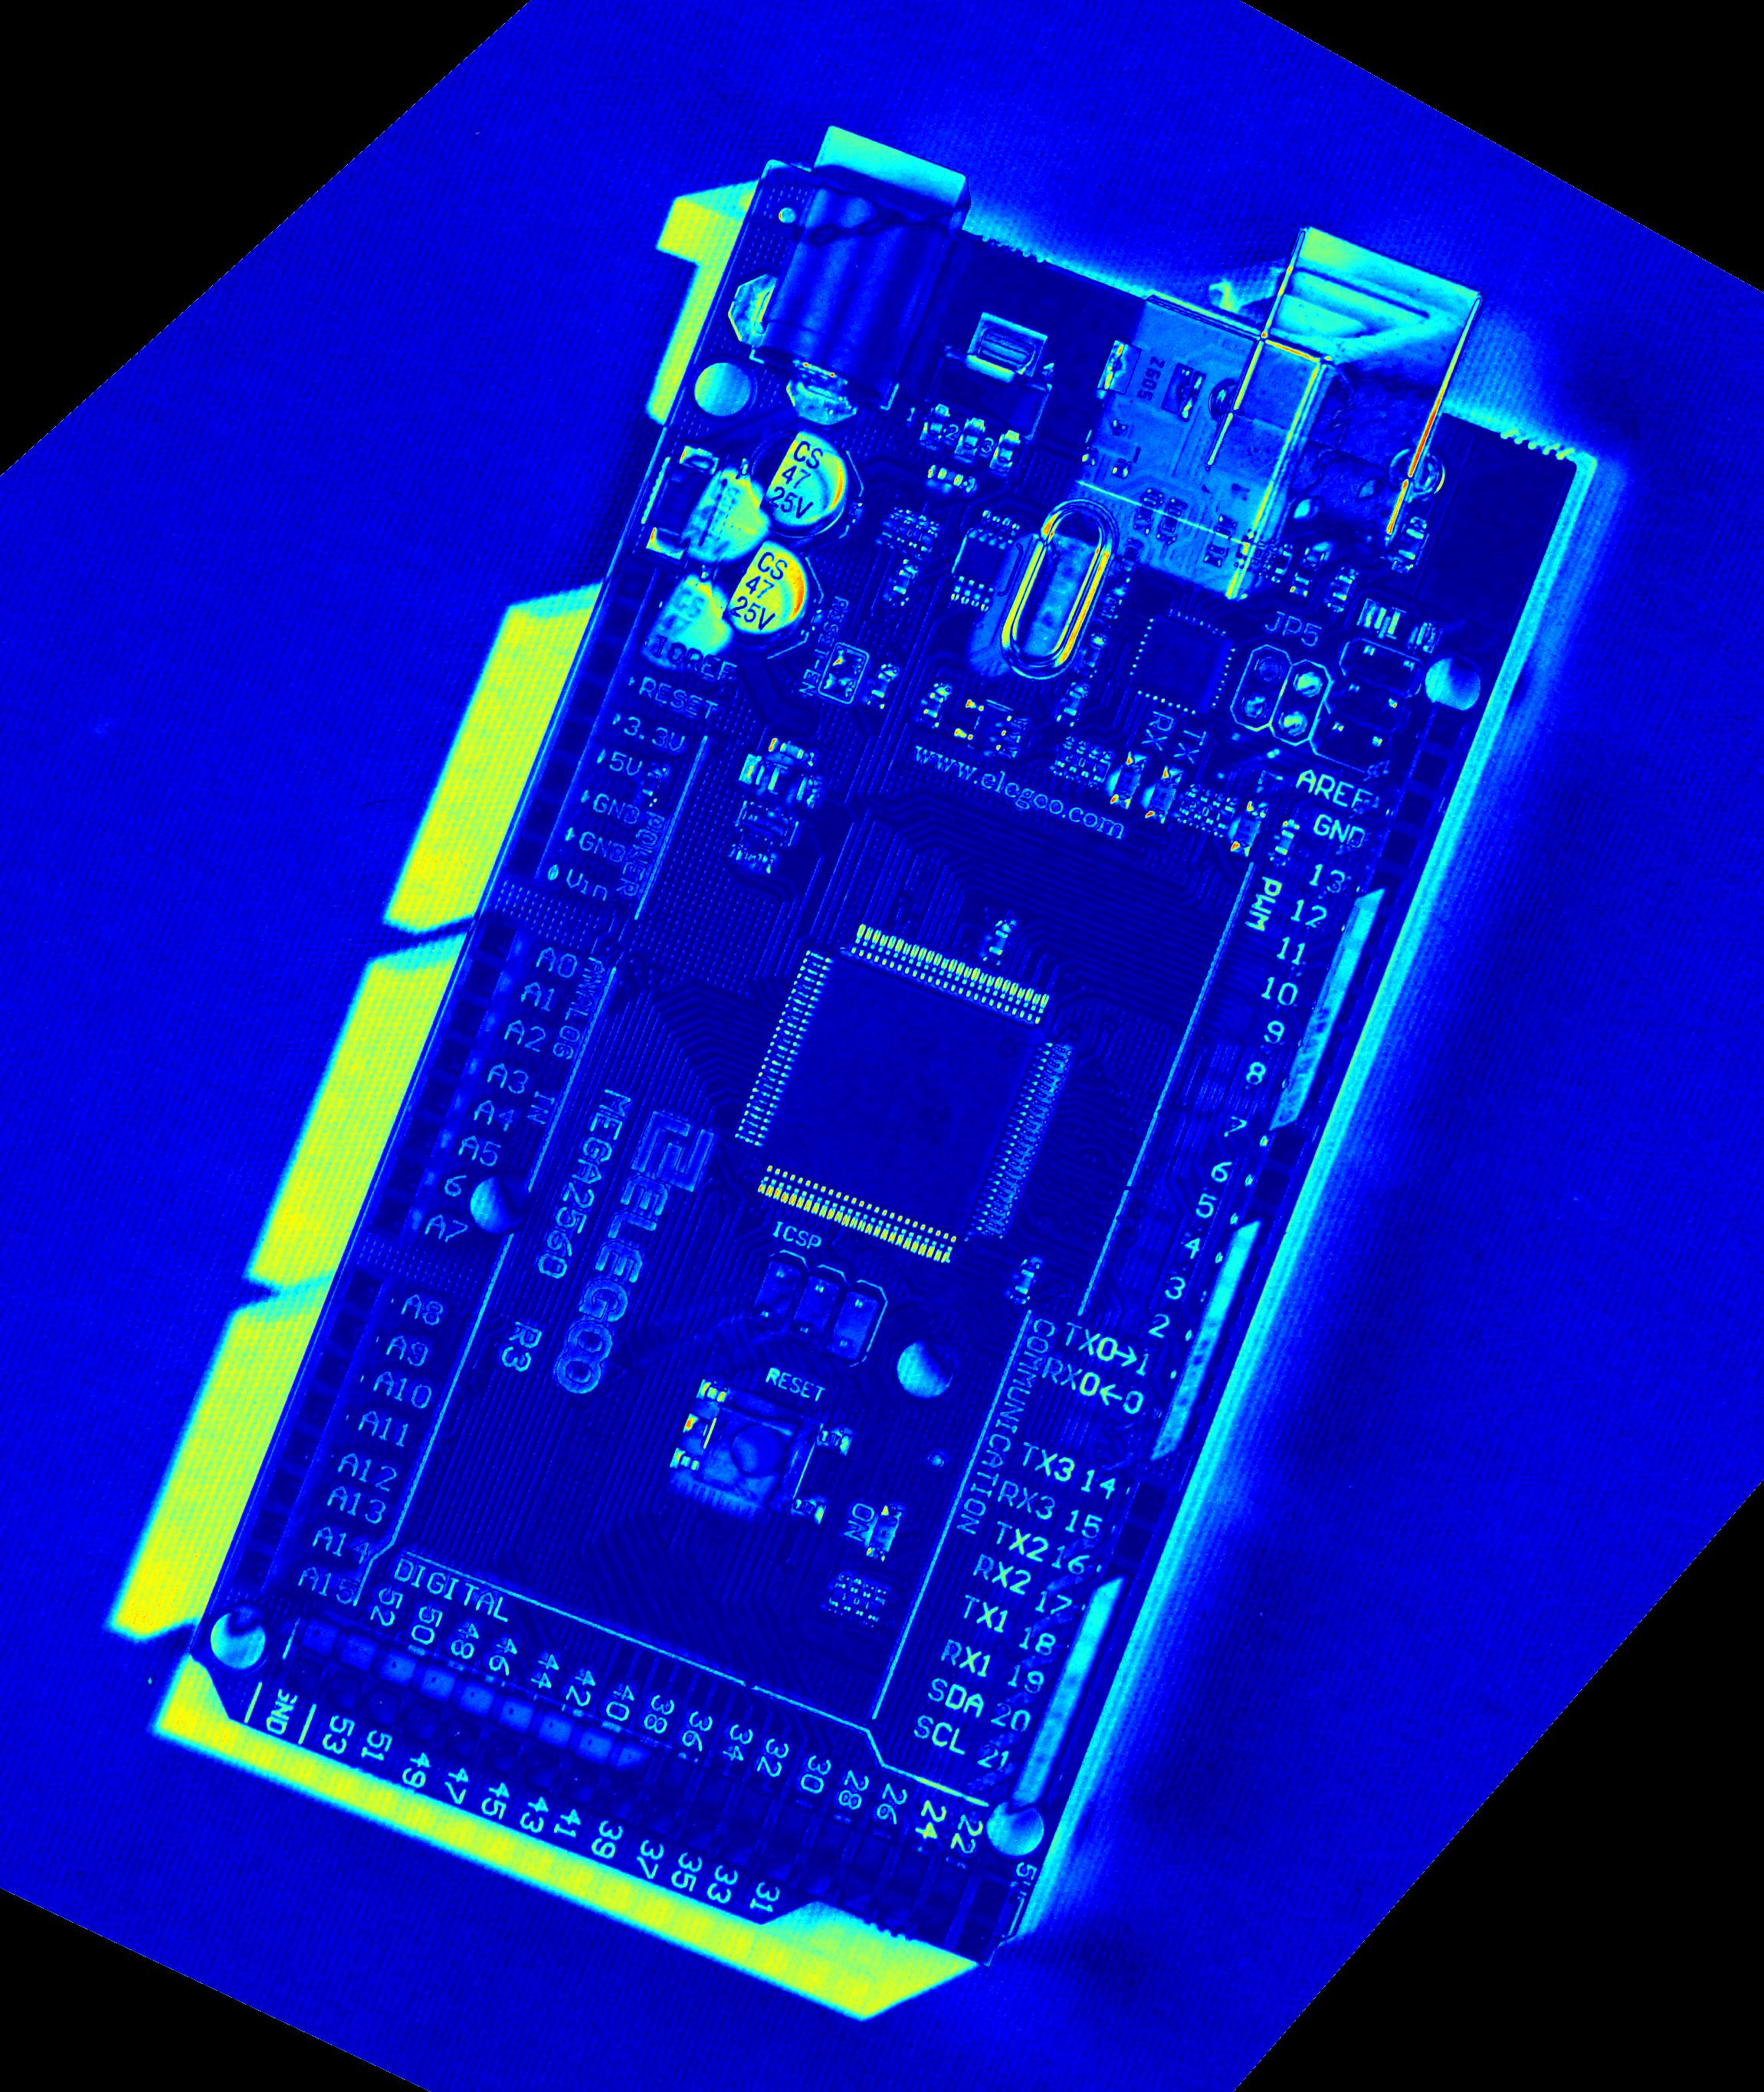
\includegraphics[height=1.38in,keepaspectratio]{report_assets/q4_heat_1.png}\\[-2pt]
{\scriptsize AAAA1}
\end{minipage}\hfill
\begin{minipage}[t]{0.32\textwidth}\centering
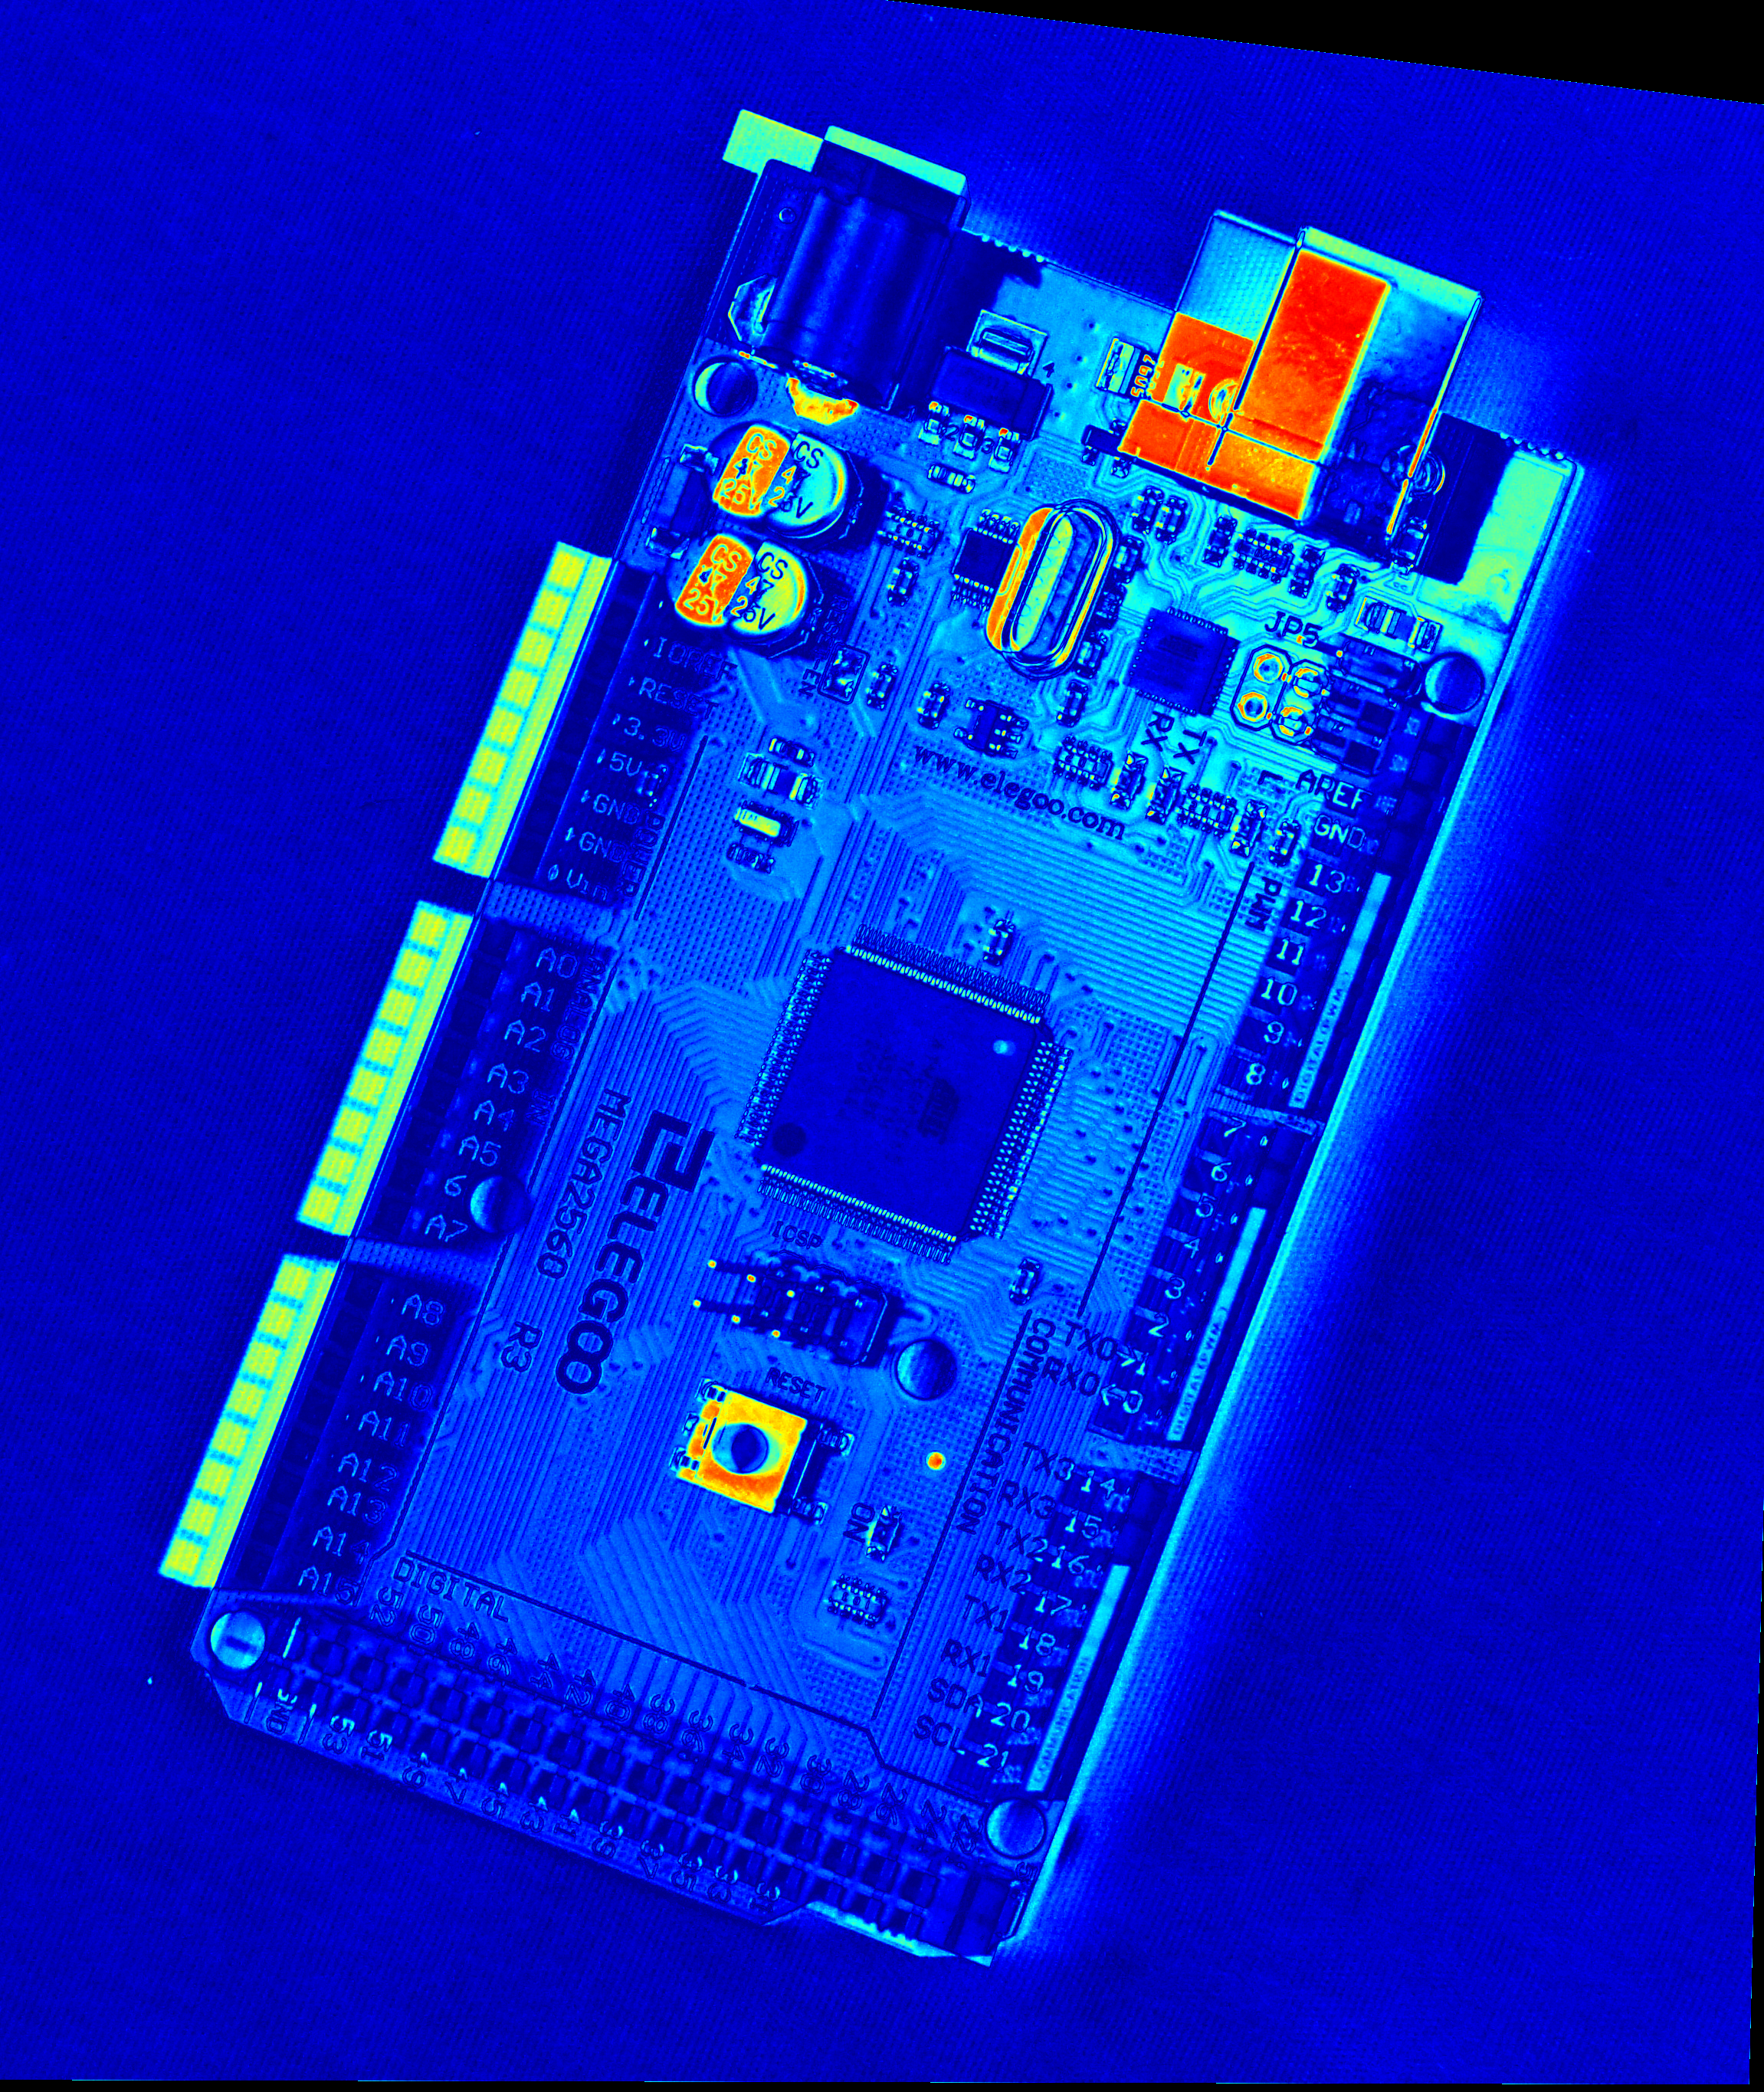
\includegraphics[height=1.38in,keepaspectratio]{report_assets/q4_heat_2.png}\\[-2pt]
{\scriptsize ADAD1}
\end{minipage}\hfill
\begin{minipage}[t]{0.32\textwidth}\centering
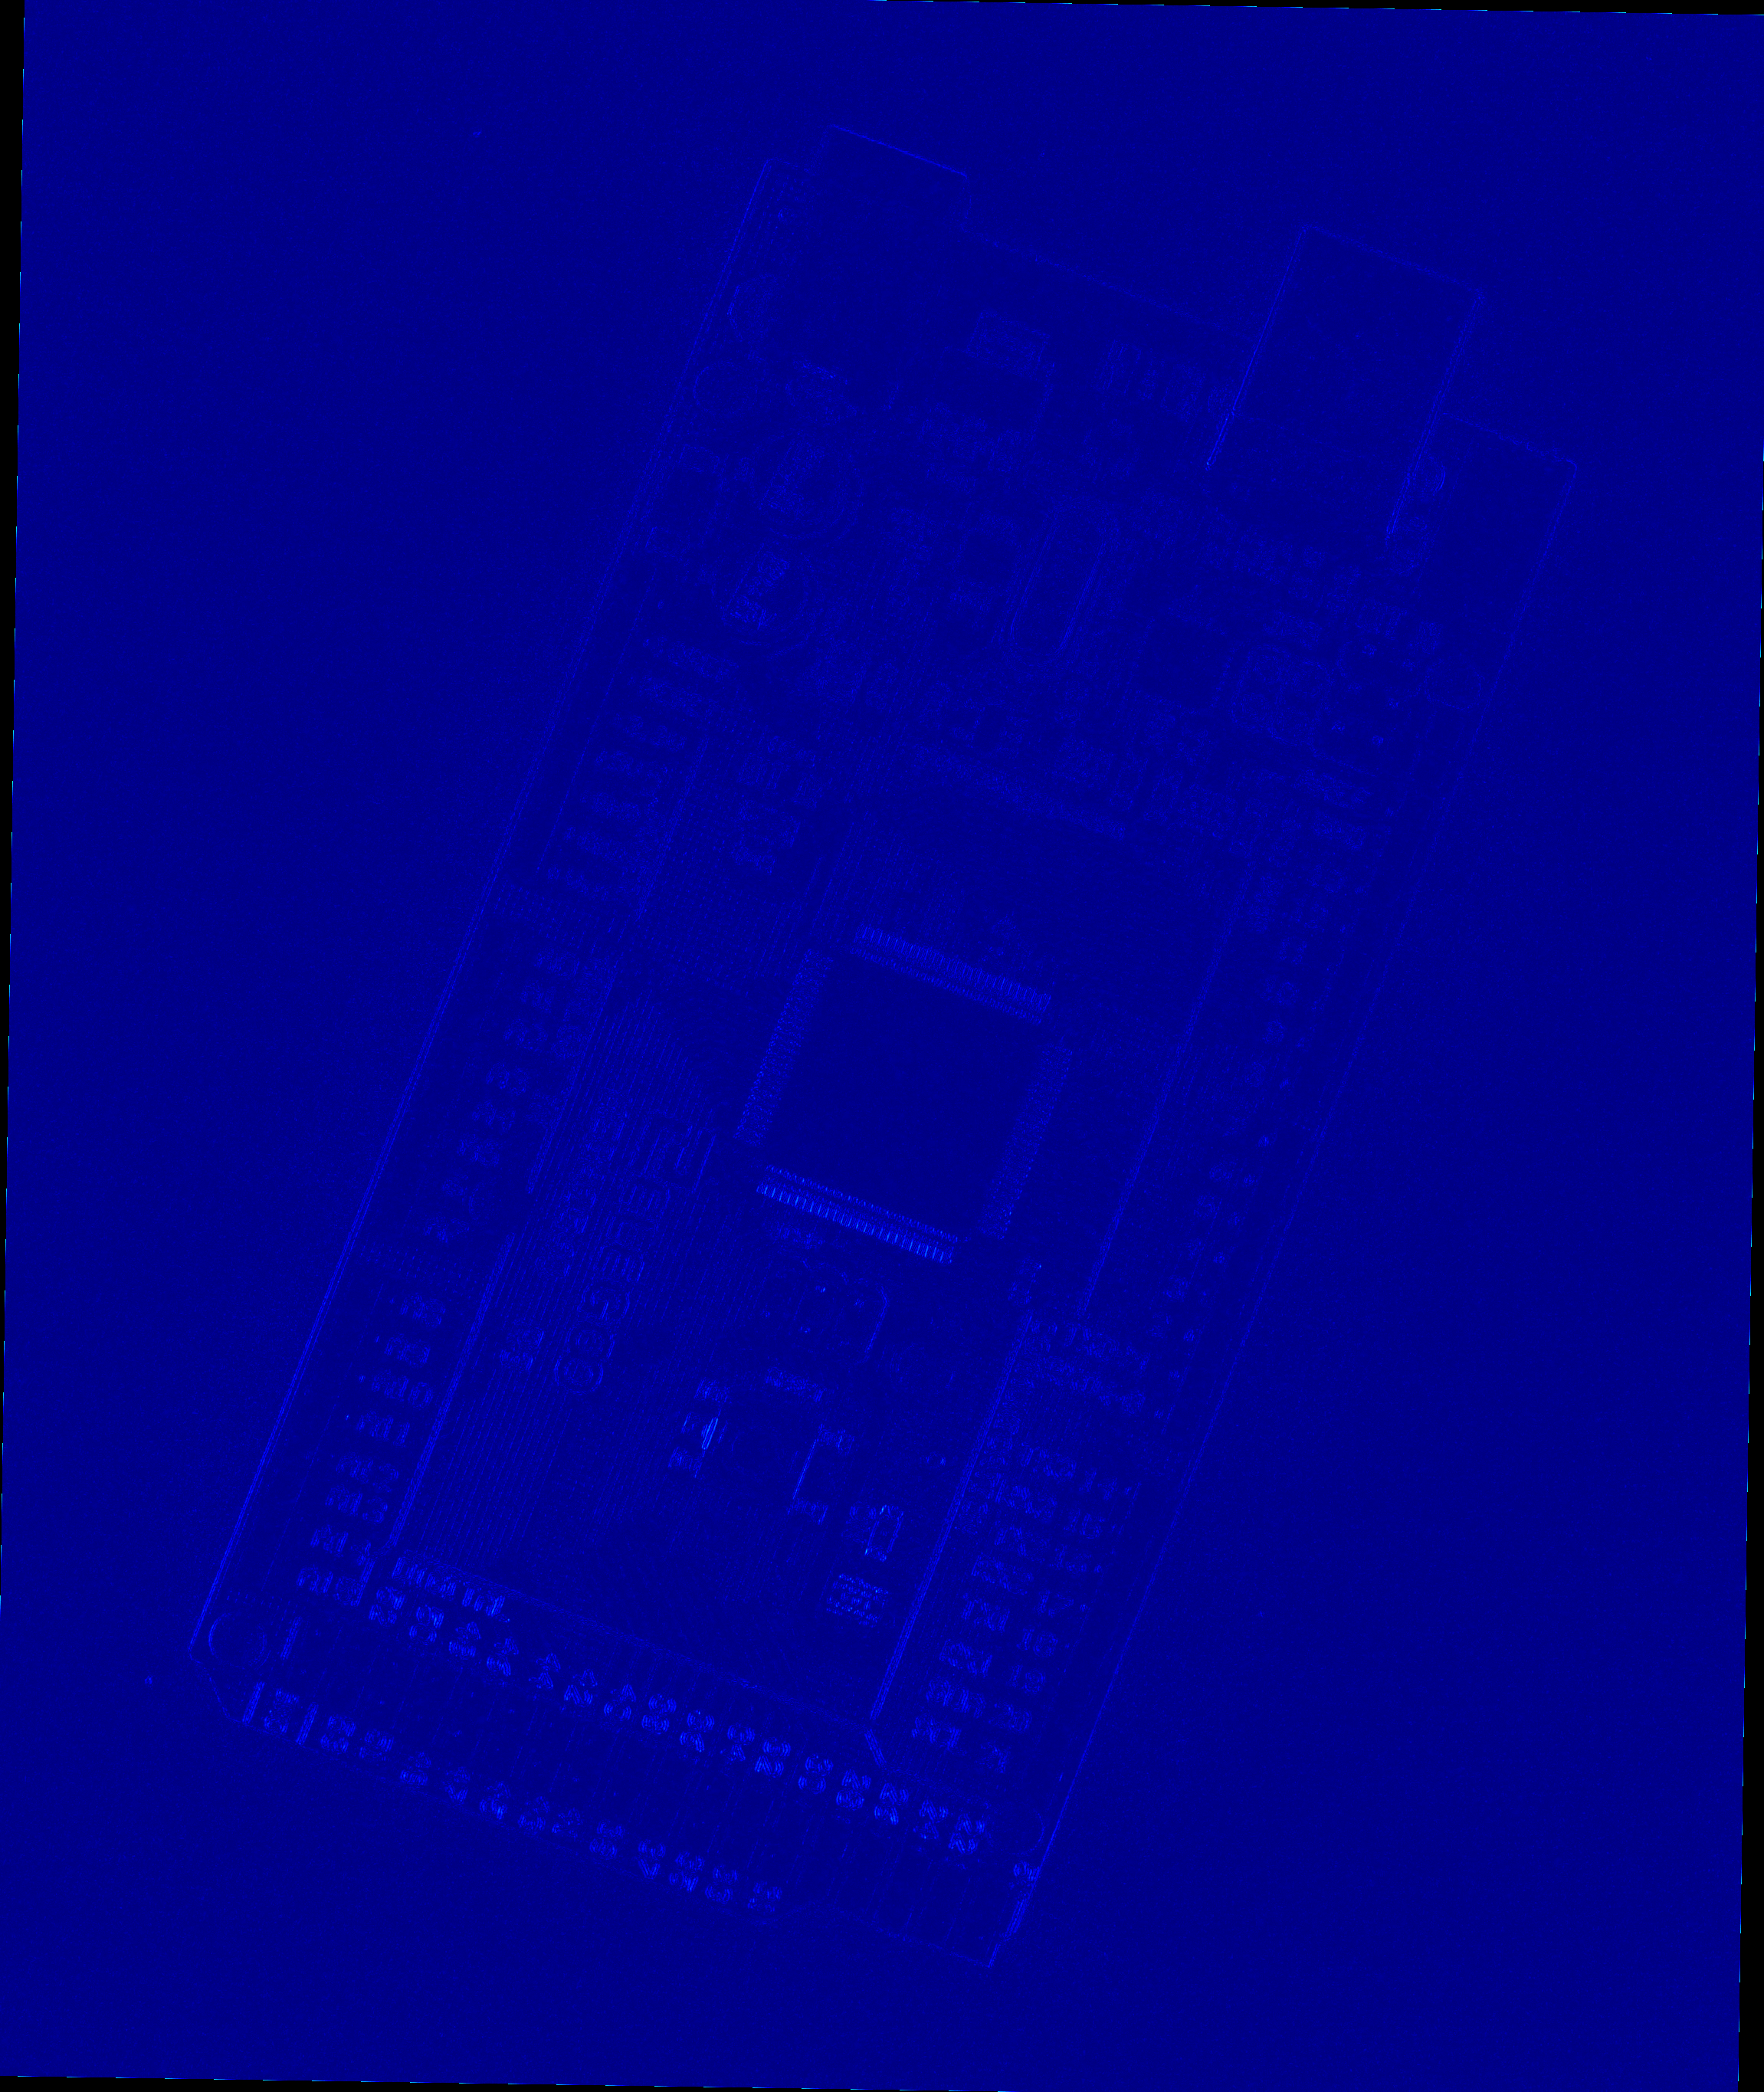
\includegraphics[height=1.38in,keepaspectratio]{report_assets/q4_heat_3.png}\\[-2pt]
{\scriptsize AECC2}
\end{minipage}

\vspace{3pt}
\makebox[\textwidth][c]{%
\begin{minipage}[t]{0.32\textwidth}\centering
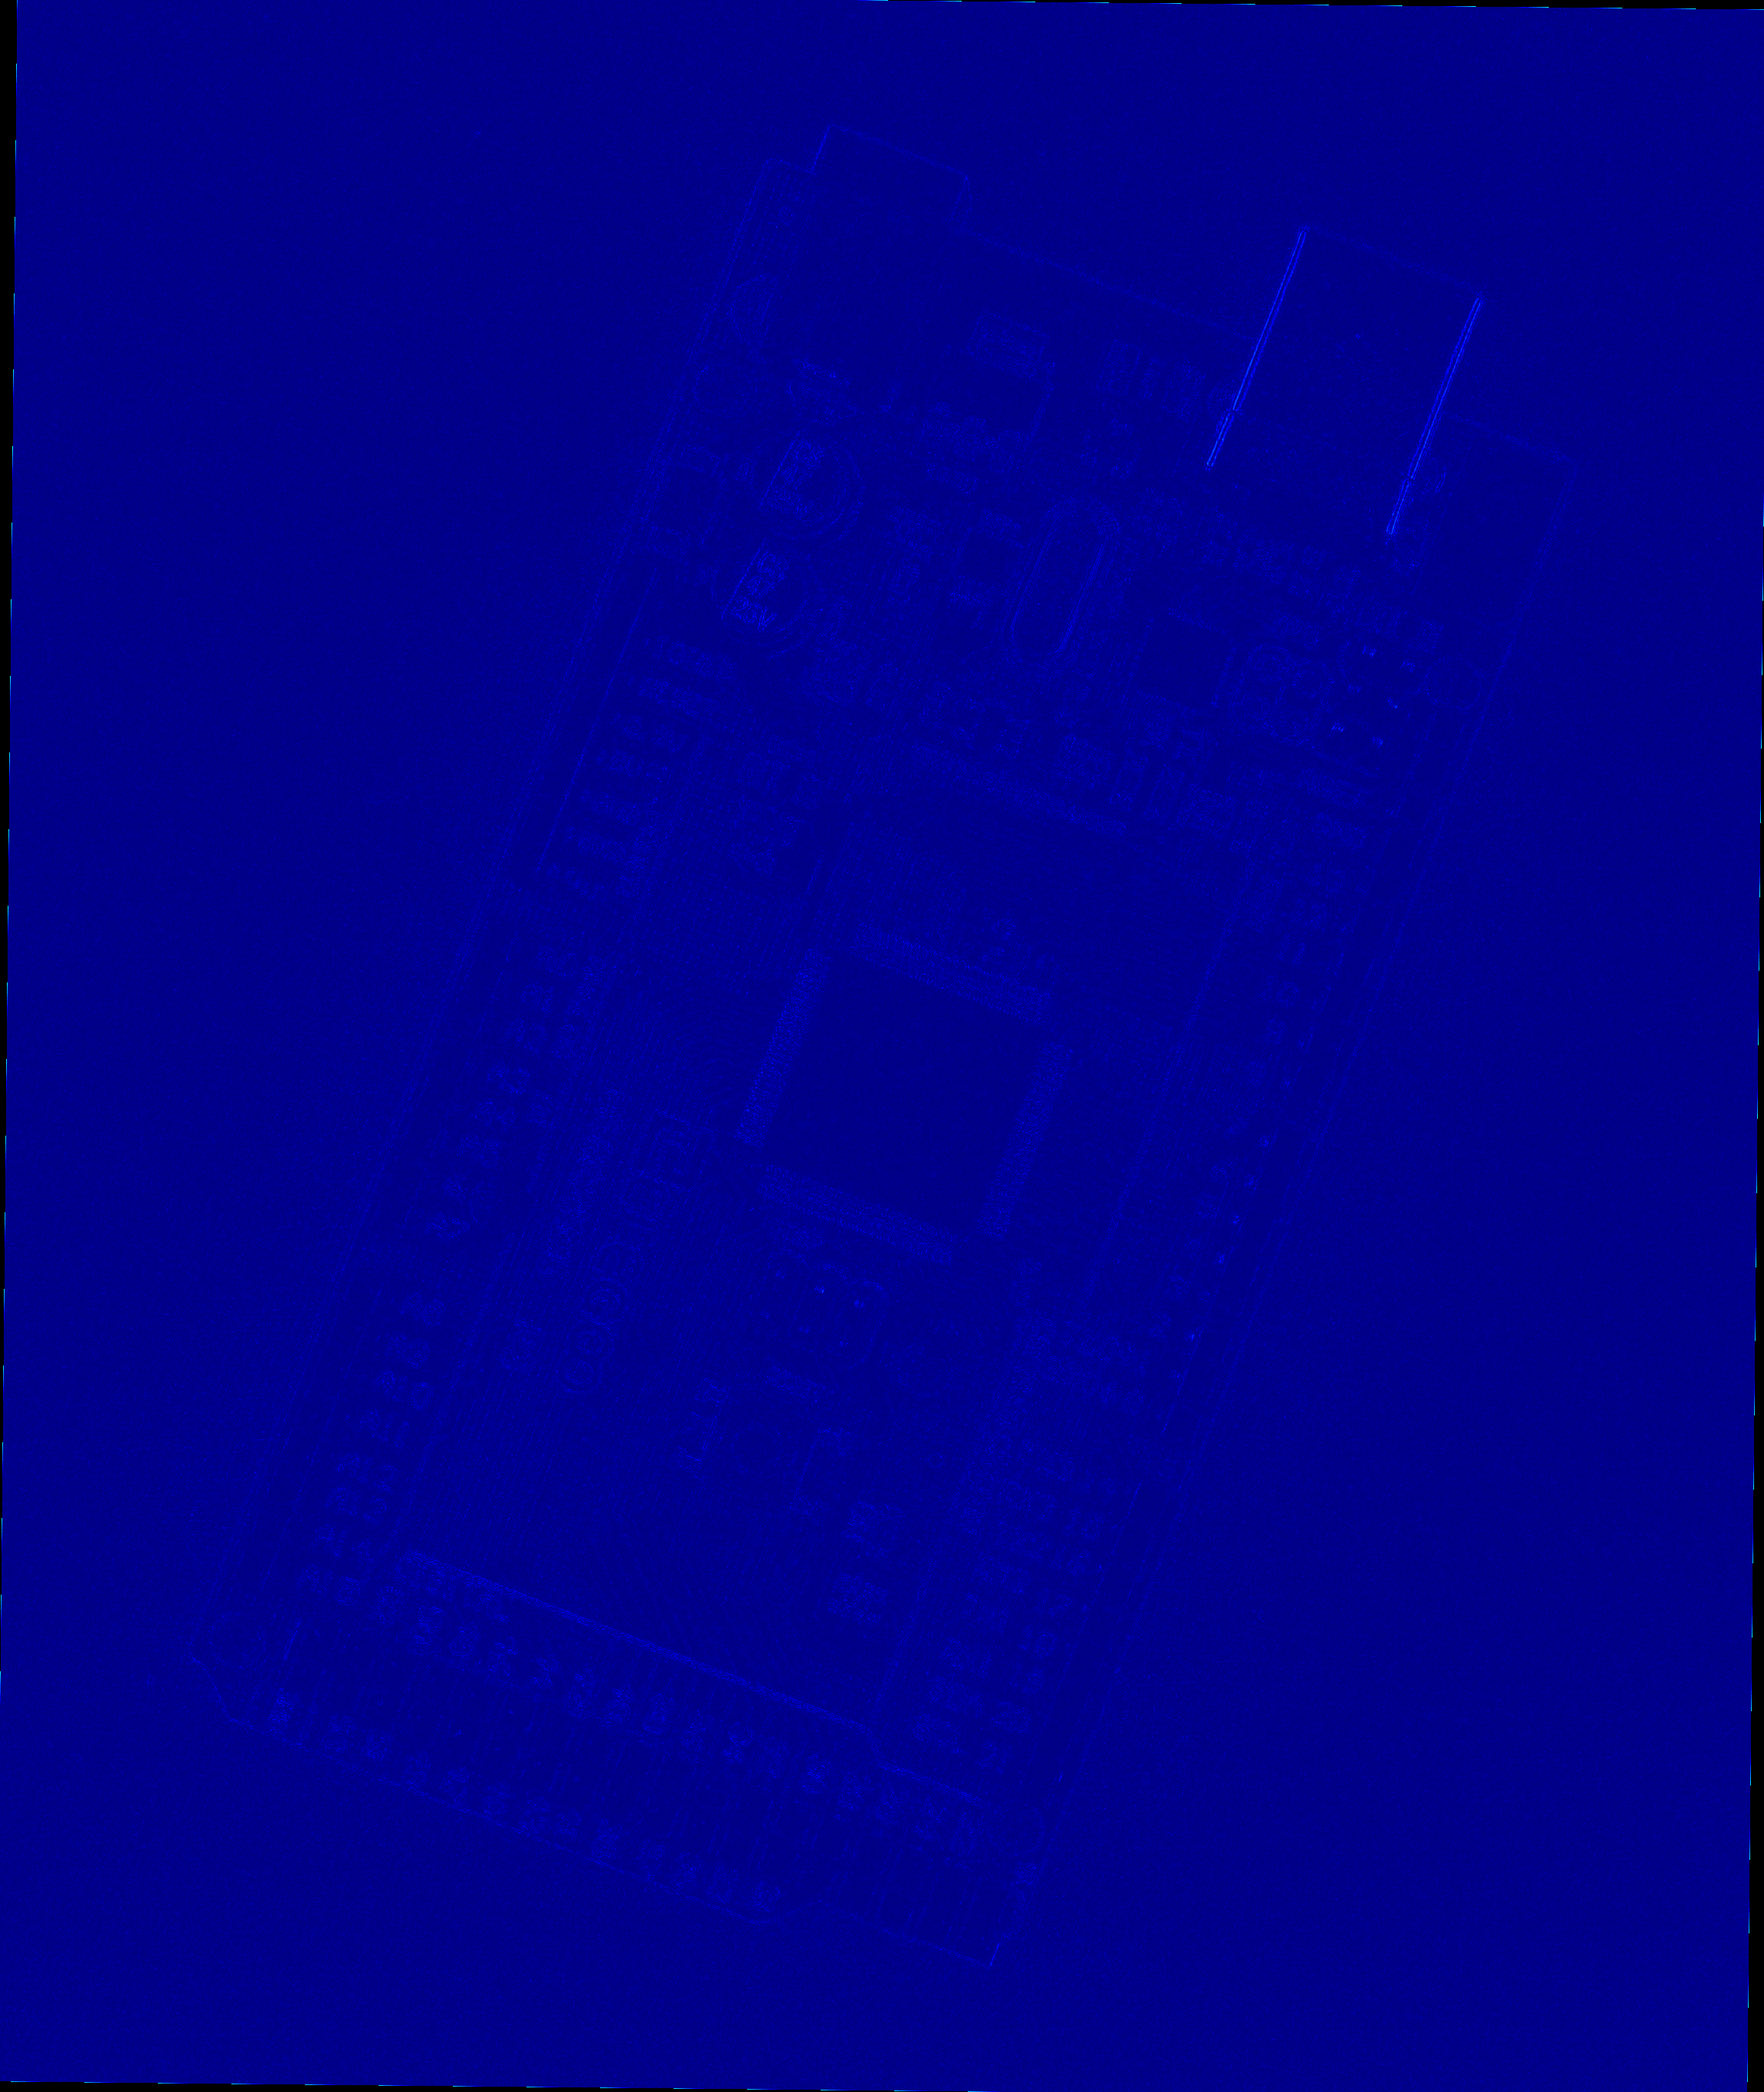
\includegraphics[height=1.38in,keepaspectratio]{report_assets/q4_heat_4.png}\\[-2pt]
{\scriptsize AECC3}
\end{minipage}\hspace{0.04\textwidth}%
\begin{minipage}[t]{0.32\textwidth}\centering
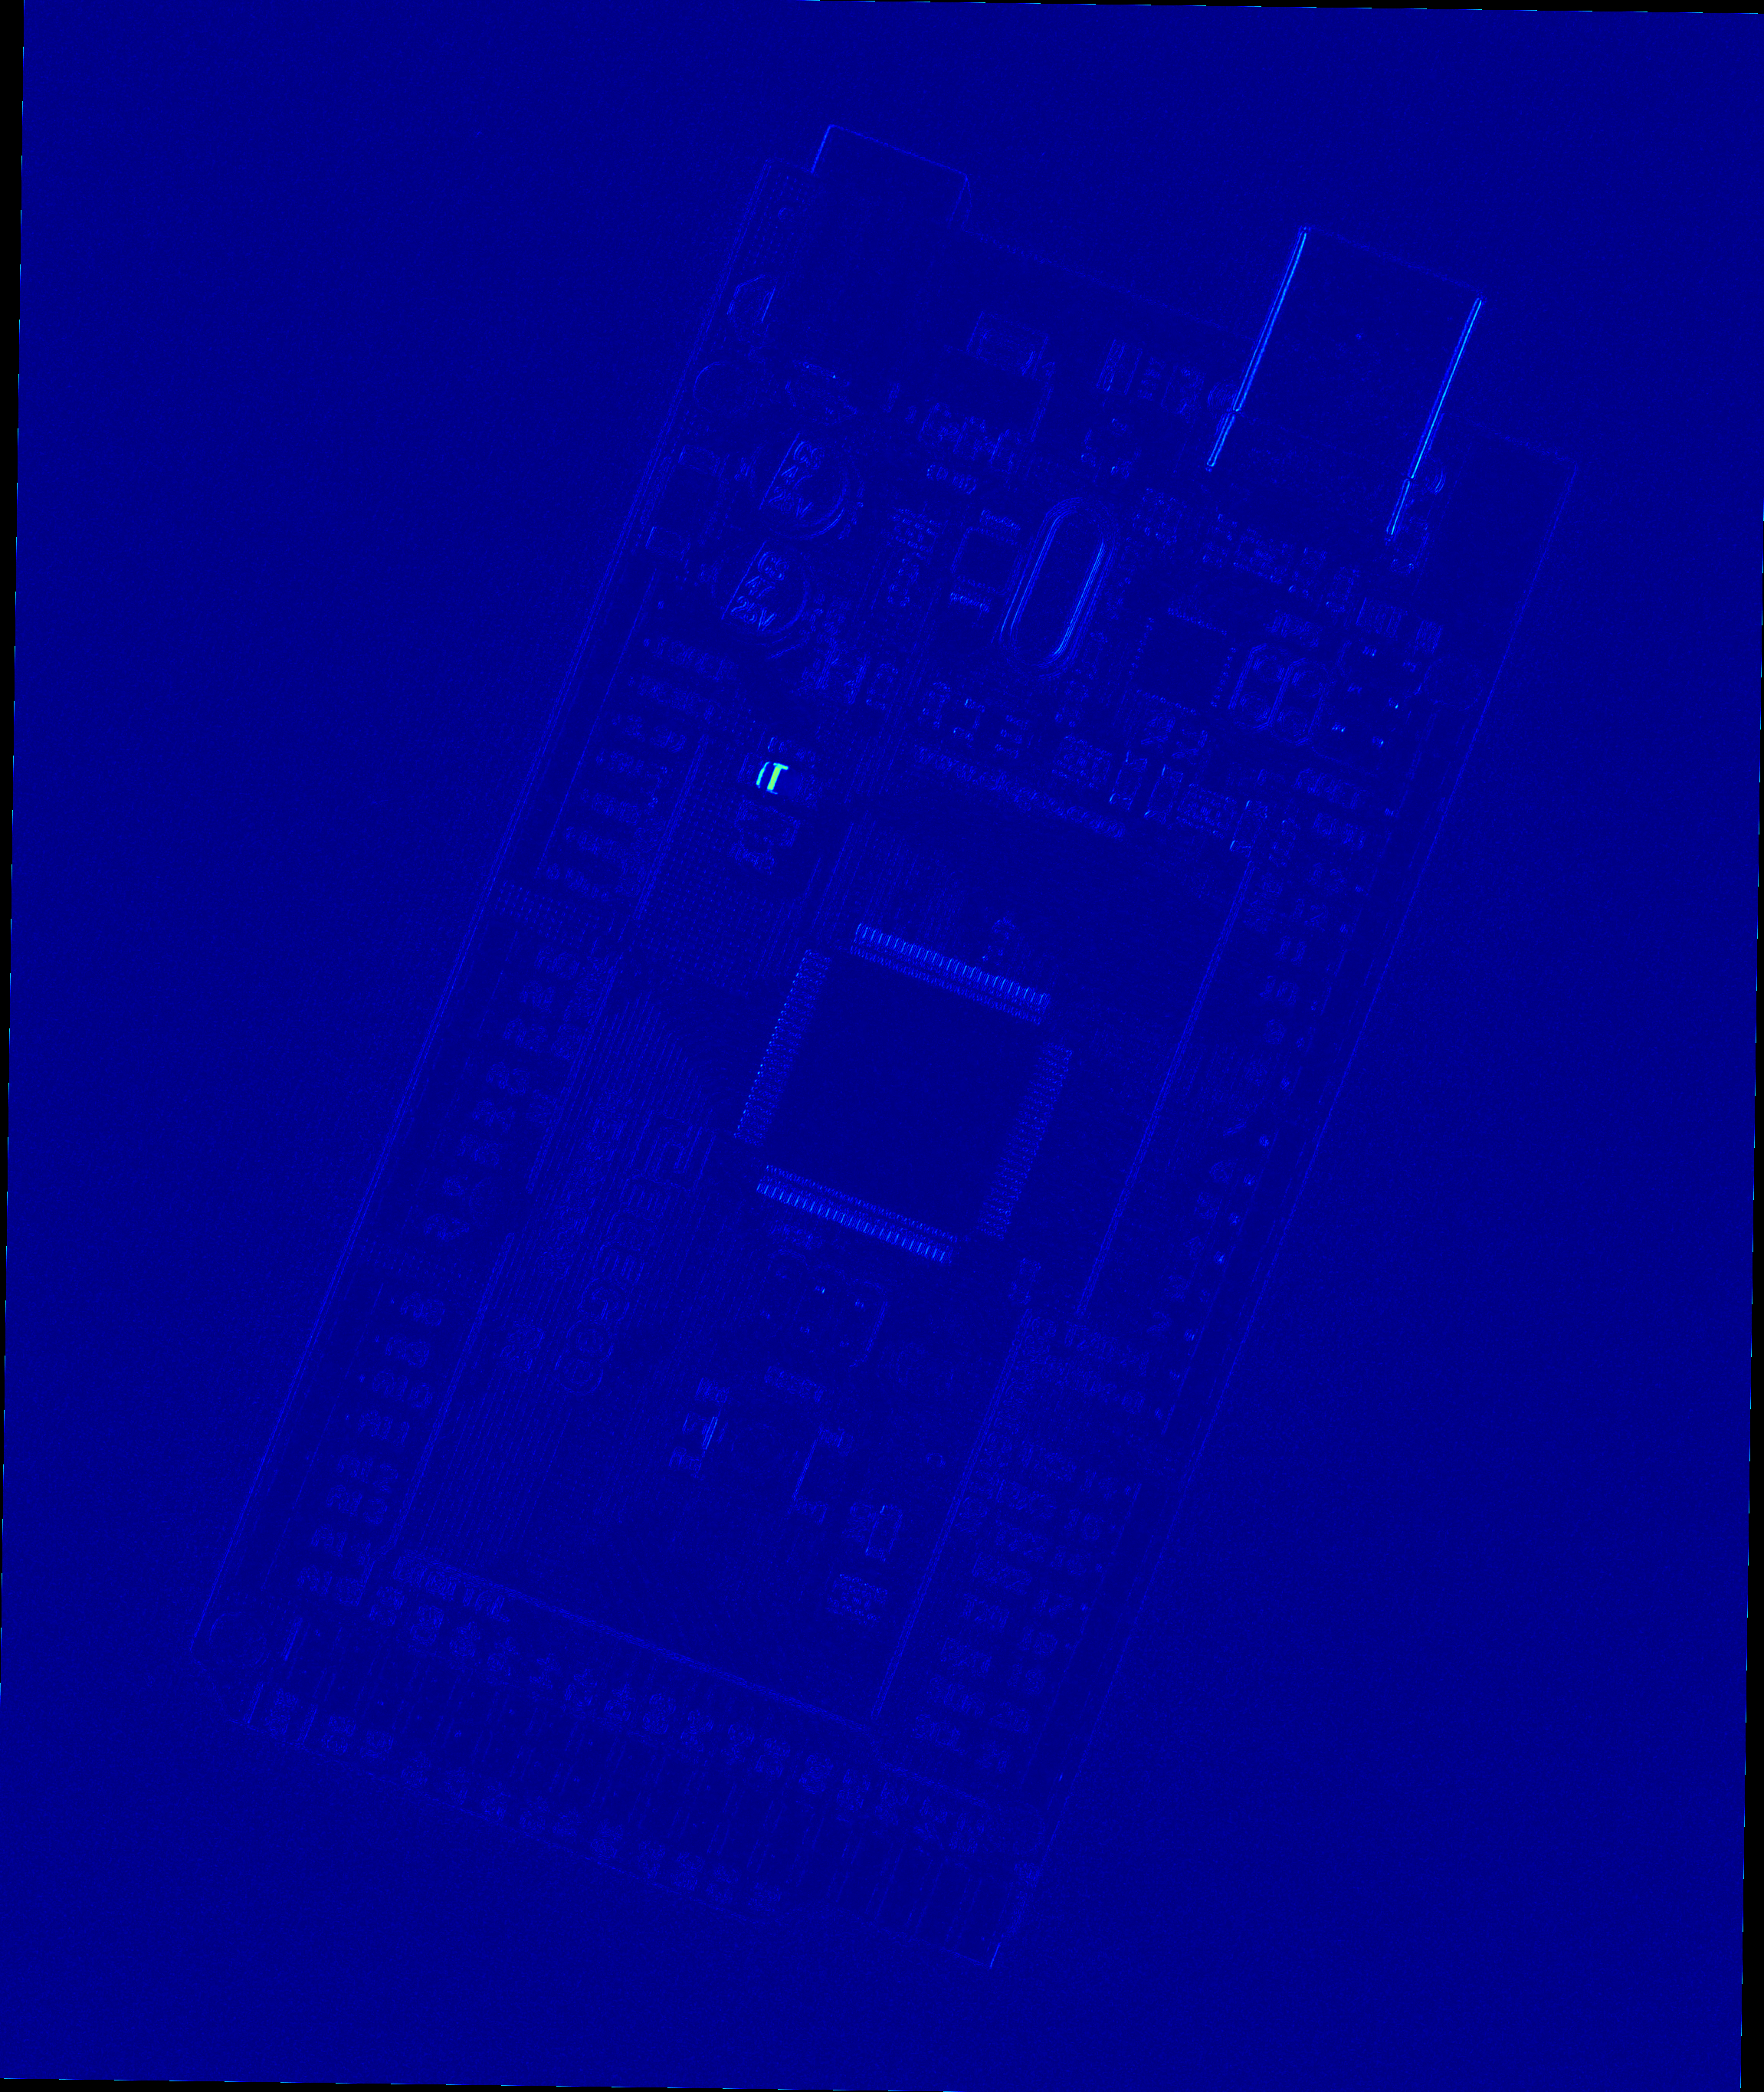
\includegraphics[height=1.38in,keepaspectratio]{report_assets/q4_heat_5.png}\\[-2pt]
{\scriptsize AECC4}
\end{minipage}}
\end{center}

\textbf{Interpretation.} \QFourHighDiffImages\ have substantially larger mean differences than AECC2--AECC4, whose mean differences are approximately $3$--$4$ grayscale levels. A high difference around a USB Type-B port, capacitors or the reset button can be caused by changed/missing components, small position or shape changes, illumination, resampling after warping, or residual registration error. A homography corrects global planar perspective but cannot remove genuine board/component differences or local parallax. Thus the difference map is a comparison aid, not by itself proof of a manufacturing fault.

\end{document}
